% !TeX spellcheck = de_DE

\chapter{Dilatation}
\label{chap:dilat}

Nach der theoretischen Beschreibung der zu entwickelnden Software, besteht das Problem, dass das Tiefenbild an manchen Stellen flimmert oder auf Grund von Reflexionen teilweise nicht dargestellt werden kann.
Um diesem Problem zu begegnen und ein hochwertigeres Tiefenbild zu erhalten, wurde die Dilatation eingesetzt.

\section{Einleitung}
In der digitalen Bildverarbeitung werden viele Verfahren zur Bildmanipulation verwendet.
Darunter auch die morphologische Bildverarbeitung.
Sie wird unter anderem zur Veränderung der Form von Bildstrukturen eingesetzt.
Im genaueren handelt es sich hierbei also um Operationen auf der Gestalt von Objekten, um diese zu verändern und Störungen zu beseitigen.

\section{Motivation}
Durch das Auftreten von Löchern in der Bildstruktur der Tiefenbildkamera ist es nötig, Bildmanipulationen durchzuführen um die Qualität zu verbessern.
Die Basis hierfür bildet die Erosion und Dilatation, welche die Basisoperationen der Bildverarbeitung darstellen.
Für unser Projekt haben wir die Dilatation verwendet, um die bestmöglichen Ergebnisse zu erzielen.
Hierbei wurde die Dilatation modifiziert, um diese auf ein Tiefenbild anwenden zu können.

\section{Dilatation}
Die Dilatation ermöglicht eine Vergrößerung von Objekten sowie das Schließen von Löchern als auch das Verbinden von Strukturen.
Durch die Verwendung eines Strukturelements wird die Formveränderung erzeugt.
Dieses Strukturelement wird nun schrittweise über das Bild gesetzt.

Hierbei wird, wie in \cref{fig:dilat_dilat} dargestellt, im Tiefenbild ein Tiefenwert gesetzt, wenn letztendlich ein Tiefenwert im Bereich des Strukturelements enthalten ist.
Der gesetzte Tiefenwert ergibt sich aus den Tiefenwerten der Nachbarschaftspixel.
\begin{figure}[H]
	\centering
	\ifthenelse{\boolean{jpg}}{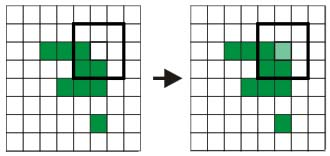
\includegraphics[width=0.5\textwidth]{dilat/dilatation.jpg}}{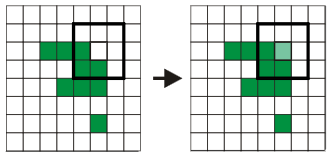
\includegraphics[width=0.5\textwidth]{dilat/dilatation.png}}
	\caption{Dilatationsoperation}
	\label{fig:dilat_dilat}
\end{figure}

\cref{fig:dilat_dilat-change} zeigt die hiermit erreichten Erfolge.

\begin{figure}[H]
	\centering
	\begin{subfigure}[t]{0.45\textwidth}
		\centering
		\ifthenelse{\boolean{jpg}}{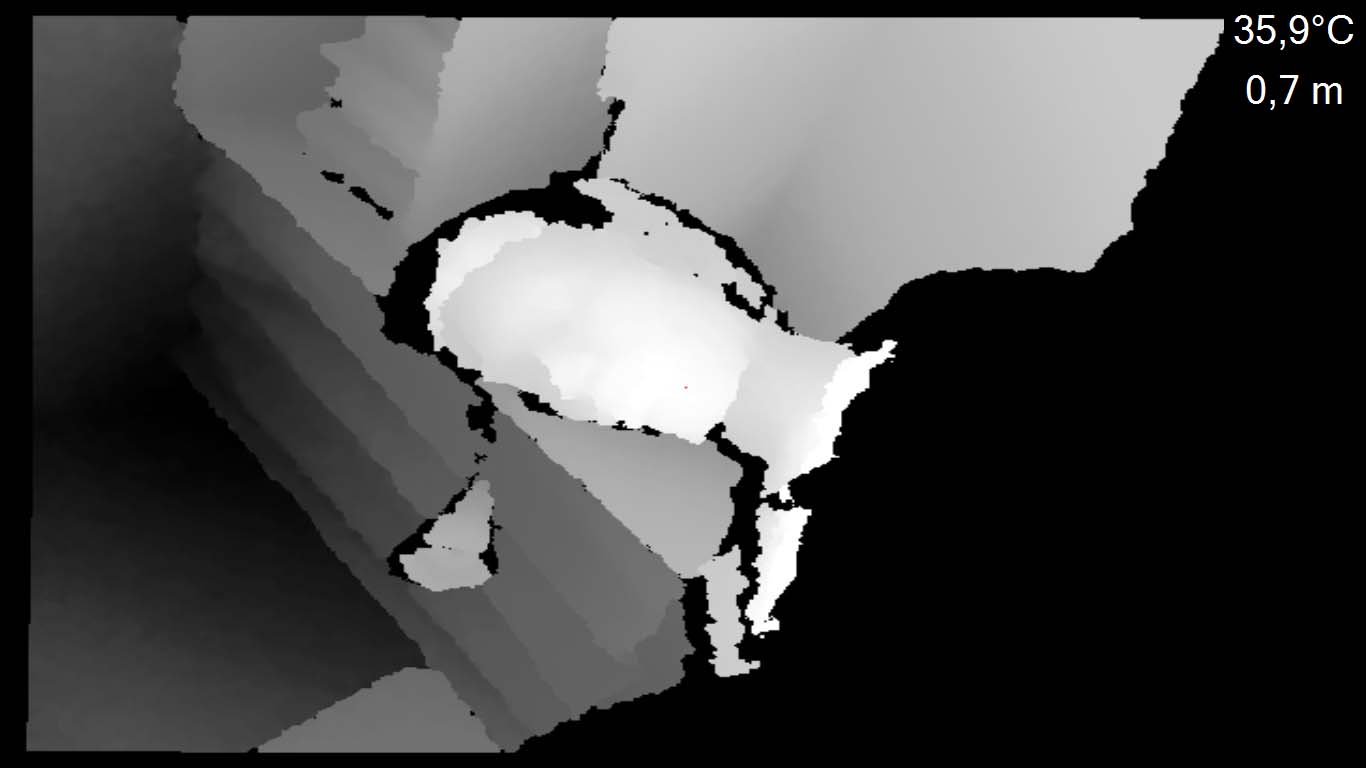
\includegraphics[width=\textwidth]{dilat/ohne-Dilatation.jpg}}{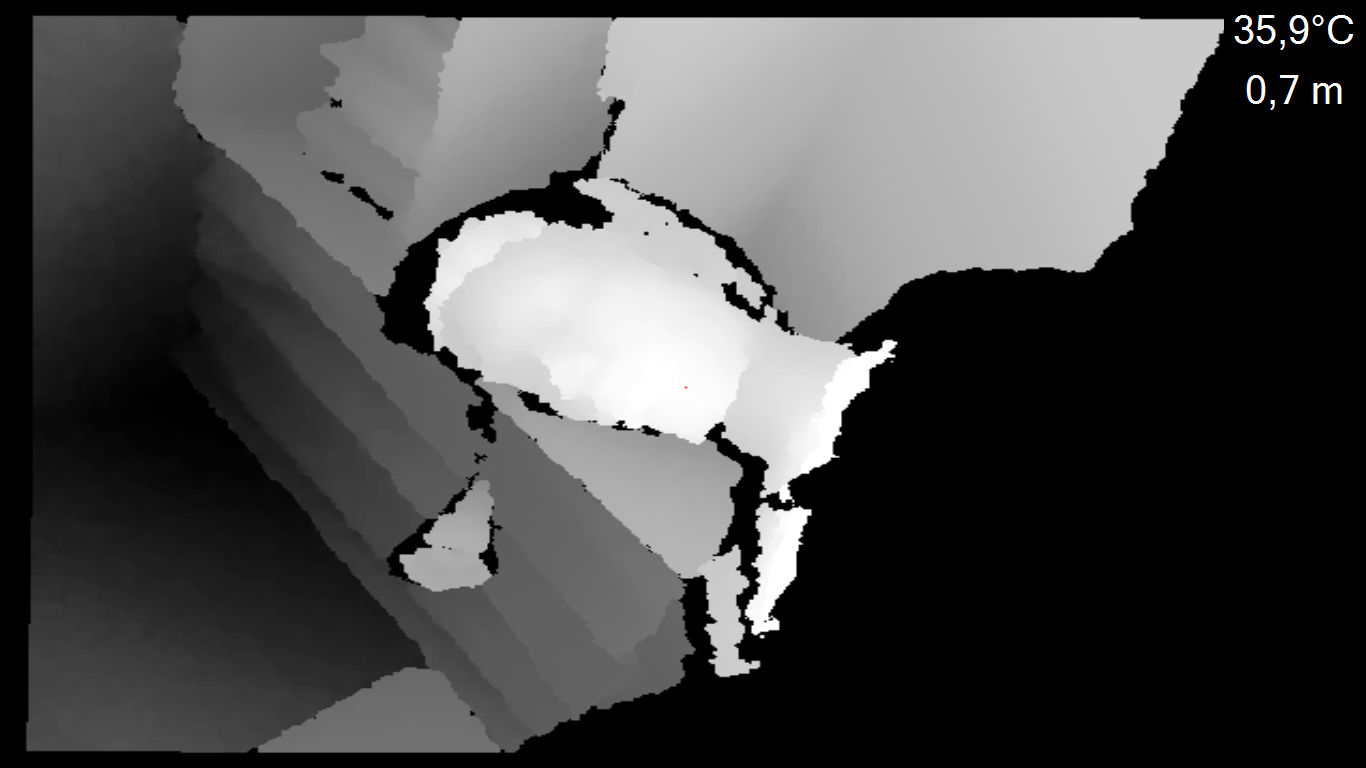
\includegraphics[width=\textwidth]{dilat/ohne-Dilatation.png}}
		\caption{Vor der Dilatation}
		\label{fig:dilat_pre}
	\end{subfigure}
	~
	\begin{subfigure}[t]{0.45\textwidth}
		\centering
		\ifthenelse{\boolean{jpg}}{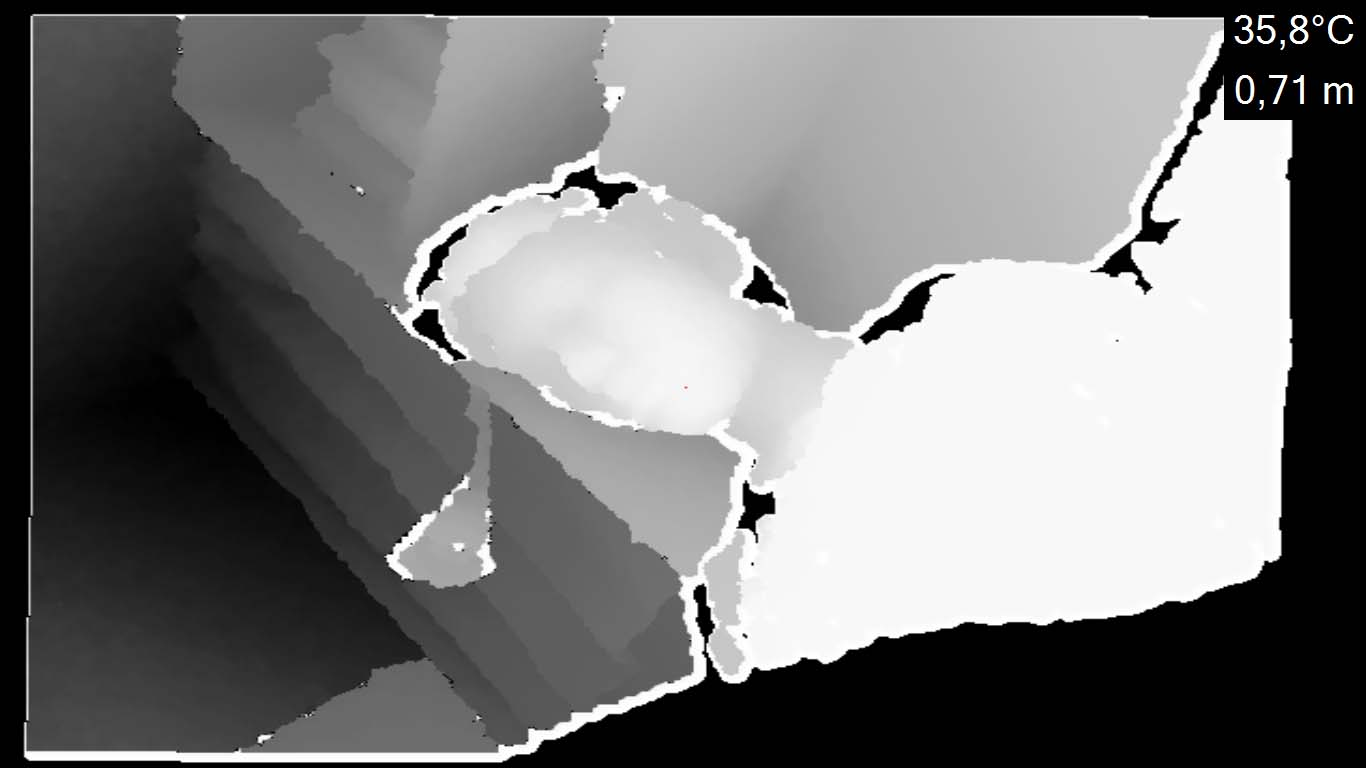
\includegraphics[width=\textwidth]{dilat/mit-Dilatation.jpg}}{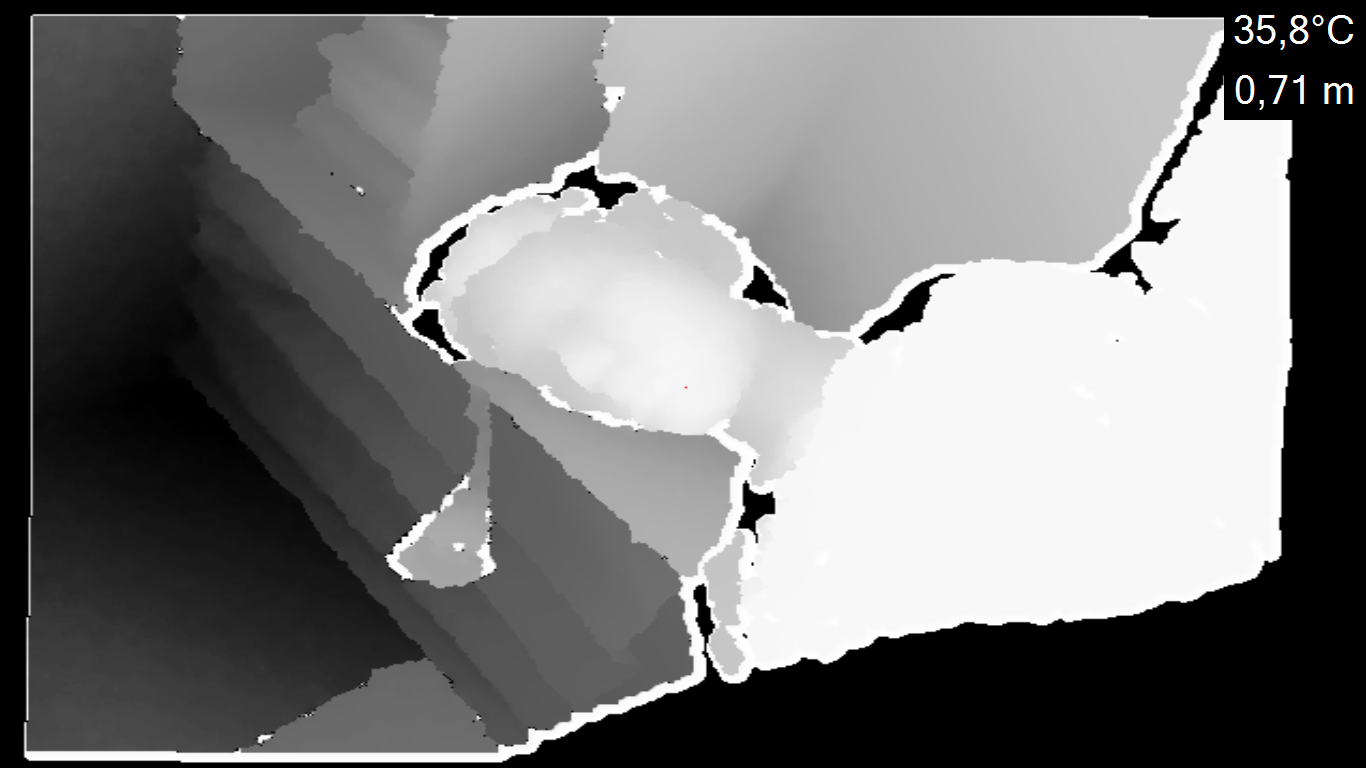
\includegraphics[width=\textwidth]{dilat/mit-Dilatation.png}}
		\caption{Nach der Dilatation}
		\label{fig:dilat_post}
	\end{subfigure}
	\caption{Effekte der Dilatation}
	\label{fig:dilat_dilat-change}
\end{figure}